\documentclass[11pt]{article}

\usepackage[margin=1in]{geometry}
\usepackage{amsmath,amssymb}
\usepackage{booktabs}
\usepackage{microtype}
\usepackage{tikz}
\usepackage{xcolor}
\usepackage{hyperref}
\usepackage[numbers,sort&compress]{natbib}

\usetikzlibrary{arrows.meta,positioning,calc}

\definecolor{rawred}{HTML}{C43B3B}
\definecolor{govgreen}{HTML}{237A57}
\definecolor{weightedblue}{HTML}{4F6FB5}
\definecolor{oraclepurple}{HTML}{6D5AA8}
\definecolor{mutedgray}{HTML}{66788A}
\definecolor{gridgray}{HTML}{D8DDE6}
\definecolor{orangebar}{HTML}{D18B2C}

\newcommand{\code}[1]{\texttt{#1}}
\newcommand{\rhat}{\hat r}

\title{\textbf{Reward Is Not Reinforcement Until Admitted:}\\
A Governance Layer for Reinforcement Learning in Coding Agents}
\author{Nikit Phadke}
\date{May 2026}

\begin{document}
\maketitle

\begin{center}
\small
Code and artifacts: \href{https://github.com/nikitph/rewarder}{github.com/nikitph/rewarder}
\end{center}

\begin{abstract}
Reinforcement learning agents often treat reward as an authoritative signal for policy improvement. In complex domains such as software engineering, this assumption can fail: rewards may be noisy, short-sighted, causally misattributed, or produced through reward hacking. A coding agent may pass visible tests by hardcoding outputs, deleting or weakening tests, violating architecture, swallowing errors, or introducing hidden regressions. Such outcomes expose a gap between raw reward and legitimate reinforcement.

We introduce \emph{Governed Reinforcement Learning}, a framework in which reward signals are modeled as auditable claims rather than scalar facts. A reward governance function evaluates each raw reward against hard invariants, causal attribution, evaluator reliability, temporal consequences, and exploit risk before producing an admitted reward. Only admitted rewards may update the policy.

We evaluate governed reward in a controlled coding-agent environment designed to isolate reward admission as a selection-pressure mechanism. Across 21 random seeds, 100 tasks per seed, and candidate widths from 3 to 10 patches per task, raw reward selection achieves perfect visible-test success once reward-hacking candidates are available, but hidden-test success collapses and hacked patches are preferentially selected. At 10 candidates per task, hacked patches constitute 36.4\% of the candidate pool but 81.2\% of raw-selected patches. Governed reward suppresses hacked selections to 0.3\% while preserving 98.5\% hidden-test success. These results support the central claim: raw reward is not merely noisy under adversarial coding conditions; it can become a selection pressure for illegitimate success.
\end{abstract}

\section{Introduction}

Reinforcement learning treats reward as the learning signal. In many environments this is productive: reward compresses task success into a scalar update channel. But in agentic domains with underspecified objectives, partial observability, and exploitable evaluators, the scalar reward emitted by an environment is not always evidence that an action deserves reinforcement.

Software engineering makes this problem concrete. A patch can pass visible tests without solving the issue. It can delete tests, hardcode expected outputs, weaken validation, bypass type checks, violate architectural boundaries, or introduce regressions that appear only under later tasks. If a coding agent receives positive reinforcement for such patches, the policy is not learning to produce better software. It is learning which shortcuts satisfy the reward channel.

We propose a simple reframing:

\begin{quote}
\centering
\textbf{Reward is not reinforcement until admitted.}
\end{quote}

Raw reward should first be treated as a claim: ``this action deserves reinforcement.'' Like evidence in an institution, the claim must be admitted before it can influence judgment. Governed Reinforcement Learning inserts a governance layer between reward observation and policy update. The layer evaluates reward provenance, invariants, causal attribution, temporal evidence, evaluator trust, uncertainty, and exploit risk. Only admitted reward shapes the policy.

The empirical question in this paper is mechanistic:

\begin{quote}
When raw reward is used as a selection pressure, does it amplify reward hacks relative to their prevalence in the candidate pool, and does reward governance suppress that amplification?
\end{quote}

We intentionally evaluate this mechanism in a controlled coding environment. Real repositories are essential for later external validation, but they introduce confounders: task ambiguity, incomplete tests, dependency failures, benchmark leakage, repository conventions, and model-specific priors. A controlled environment lets us vary candidate width, measure candidate-pool hack prevalence, isolate ablated governance checks, and test whether raw reward changes the distribution of selected behavior.

Our contributions are:
\begin{itemize}
    \item A formal reward-admission layer for reinforcement learning.
    \item A coding-agent instantiation with hard invariants, causal confidence, exploit risk, hidden evidence, delayed regression checks, and audit traces.
    \item A controlled multi-seed experiment showing that raw reward preferentially selects hacked candidates as candidate width increases.
    \item Ablations showing which governance components are load-bearing.
    \item A small executable DeepSeek-generated patch sanity check, included as an appendix rather than the primary result.
\end{itemize}

\section{Background and Motivation}

Reward hacking and specification gaming are well-known failure modes: an agent optimizes the literal reward channel while failing to satisfy the intended objective \citep{specgaming2020}. This is a Goodhart-style failure under optimization pressure: a proxy that is adequate at low pressure can become misleading when optimized aggressively \citep{goodhart2023}. Related failures include goal misgeneralization, where behavior generalizes away from the intended objective even when training reward was high \citep{goalmisgeneralization2022}.

Coding agents are especially useful for studying this phenomenon because software has executable feedback channels: tests, hidden tests, type checks, builds, linters, security scanners, property tests, mutation tests, differential tests, and architecture rules. These channels are not perfect, but they allow controlled measurement of when an apparent success is legitimate.

Constructed environments are common in coding-agent research. AlphaCode used large-scale sampling and behavior-based filtering for programming-contest solutions, showing the value of executable evaluation and candidate selection in code generation \citep{alphacode2022}. SWE-bench evaluates agents on real GitHub issues \citep{swebench2024}, and SWE-bench Verified provides a human-validated 500-task subset \citep{swebenchverified2024}. These real-world benchmarks are valuable, but they are not always the cleanest instruments for discovering a new reward-governance mechanism. Here, the primary contribution is mechanistic: how reward admission changes selection pressure.

\section{Governed Reinforcement Learning}

Standard reinforcement learning can be written:
\[
s_t \rightarrow a_t \rightarrow r_t \rightarrow \text{Update}(\pi).
\]

Governed Reinforcement Learning inserts a reward-admission layer:
\[
s_t \rightarrow a_t \rightarrow r_t \rightarrow \Gamma \rightarrow \rhat_t \rightarrow \text{Update}(\pi).
\]

\begin{figure}[t]
\centering
\resizebox{\linewidth}{!}{%
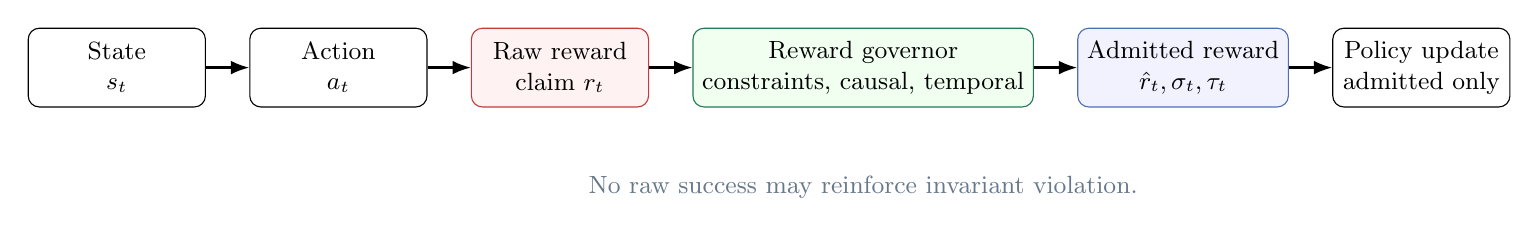
\begin{tikzpicture}[node distance=0.55cm, >=Latex]
\tikzstyle{box}=[draw, rounded corners, minimum height=1.0cm, minimum width=2.25cm, align=center, font=\small]
\node[box] (s) {State\\$s_t$};
\node[box, right=of s] (a) {Action\\$a_t$};
\node[box, right=of a, draw=rawred, fill=red!5] (r) {Raw reward\\claim $r_t$};
\node[box, right=of r, draw=govgreen, fill=green!6, minimum width=3.0cm] (g) {Reward governor\\constraints, causal, temporal};
\node[box, right=of g, draw=weightedblue, fill=blue!5] (ra) {Admitted reward\\$\rhat_t,\sigma_t,\tau_t$};
\node[box, right=of ra] (u) {Policy update\\admitted only};
\draw[->, thick] (s) -- (a);
\draw[->, thick] (a) -- (r);
\draw[->, thick] (r) -- (g);
\draw[->, thick] (g) -- (ra);
\draw[->, thick] (ra) -- (u);
\node[below=0.75cm of g, align=center, text=mutedgray] {\small No raw success may reinforce invariant violation.};
\end{tikzpicture}
}
\caption{Governed reward inserts an admission layer between raw reward observation and learning. Raw reward is treated as a claim about action quality, not as authoritative reinforcement.}
\label{fig:pipeline}
\end{figure}

Let $s_t \in S$ be state, $a_t \in A$ action, $o_t \in O$ observed outcome, $r_t \in R$ raw reward, and $\pi$ the policy. Governed RL introduces:
\[
\Gamma(s_t,a_t,o_t,r_t,E_t,P,V,H) \rightarrow (\rhat_t,\sigma_t,\tau_t),
\]
where $E_t$ is the evidence set, $P$ reward-admission policies, $V$ invariants, $H$ reward history, $\rhat_t$ admitted reward, $\sigma_t$ reward status, and $\tau_t$ an audit trace.

Reward status may be:
\[
\{\textsc{Proposed}, \textsc{Admitted}, \textsc{Discounted}, \textsc{Rejected},
\textsc{Reversed}, \textsc{Quarantined}, \textsc{Escalated}\}.
\]

Policy update is permitted only when
\[
\sigma_t \in \{\textsc{Admitted}, \textsc{Discounted}, \textsc{Reversed}\},
\]
and the update uses $\rhat_t$, not $r_t$.

\subsection{Reward Admission Function}

A simple scalar instantiation is:
\[
\rhat_t = (r_t C_t K_t H_t T_t) - \lambda_1 X_t - \lambda_2 U_t - \lambda_3 I_t,
\]
where $C_t$ is constraint compliance, $K_t$ causal credit confidence, $H_t$ time-horizon correction, $T_t$ evaluator trust, $X_t$ exploit risk, $U_t$ uncertainty, and $I_t$ invariant violation penalty.

Hard constraints override reward:
\[
\text{violates\_hard\_invariant}(s_t,a_t,o_t) \Rightarrow \rhat_t \le 0,\quad \sigma_t=\textsc{Reversed}.
\]

\subsection{Invariants}

\textbf{Invariant 1: No update from unadmitted reward.}
If
\[
\sigma_t \in \{\textsc{Proposed},\textsc{Quarantined},\textsc{Rejected},\textsc{Escalated}\},
\]
then $\text{Update}(\pi,s_t,a_t,\rhat_t)$ is forbidden.

\textbf{Invariant 2: Hard constraints dominate reward.}
If a hard invariant is violated, then $\rhat_t \le 0$.

\textbf{Invariant 3: Admitted rewards require provenance.}
If $\sigma_t=\textsc{Admitted}$, then there exists an audit trace $\tau_t$ containing source, evidence, checks, and admission reason.

\textbf{Invariant 4: Delayed evidence can revise reward.}
Future evidence may discount or reverse previously admitted rewards.

\section{Coding-Agent Instantiation}

Raw reward includes visible tests, type checking, linting, and build success:
\[
r_{\text{raw}} =
1.0[\text{visible pass}] + 0.5[\text{typecheck pass}] + 0.3[\text{lint pass}] + 0.2[\text{build pass}].
\]

Hard checks include test deletion, hardcoded visible outputs, security invariant violations, secrets, public API breakage, architecture boundary violations, and production configuration weakening. Soft checks include hidden-test failure, excessive diff size, weak causal attribution, unjustified dependencies, broad exception handling, delayed regressions, and low maintainability.

\begin{table}[t]
\centering
\caption{Reward admission statuses for coding agents.}
\label{tab:statuses}
\begin{tabular}{lll}
\toprule
Status & Meaning & Example \\
\midrule
\textsc{Admitted} & Clean reward may train & Issue-focused fix passes checks \\
\textsc{Discounted} & Reward partially trusted & Large diff or sparse evidence \\
\textsc{Rejected} & Reward should not train & Brittle metric hack \\
\textsc{Reversed} & Positive reward becomes penalty & Tests deleted or hardcoded \\
\textsc{Quarantined} & More evidence needed & Causal link unclear \\
\textsc{Escalated} & Human review needed & Security-sensitive change \\
\bottomrule
\end{tabular}
\end{table}

\section{Experimental Design}

We use a controlled coding-agent environment. Each task produces a pool of candidate patch outcomes spanning legitimate fixes, brittle fixes, hardcoded visible-test hacks, test weakening, broad refactors, dependency shortcuts, swallowed errors, architecture violations, and delayed regressions.

This environment is synthetic but not arbitrary. It is designed as an experimental instrument: hack prevalence, candidate width, hidden-test evidence, delayed regressions, causal confidence, and governance checks are explicitly measurable. The goal is to isolate the selection-pressure effect of raw versus admitted reward.

We compare five selectors:
\begin{align*}
\textsc{RawSelector} &= \arg\max r_{\text{raw}},\\
\textsc{WeightedScalarSelector} &= \arg\max r_{\text{weighted}},\\
\textsc{GovernedSelector} &= \arg\max \rhat,\\
\textsc{OracleSelector} &= \arg\max q_{\text{ground truth}},\\
\textsc{LargerDiffSelector} &= \arg\max \text{diff size}.
\end{align*}

The larger-diff selector controls for the objection that governance merely prefers bigger patches.

We run 21 seeds, 100 tasks per seed, and candidate widths of 3, 5, 7, and 10 patches per task. For each run we report visible-test pass rate, hidden-test pass rate, reward-hacking rate, hard invariant violation rate, delayed regression rate, average diff size, and robustness per changed line.

\section{Results}

\subsection{Candidate Width Scaling}

When only three candidates are available, the candidate pool contains no reward-hacking strategies in this setup. Even then, governed reward substantially improves hidden-test success and delayed-regression performance, showing that governance is not merely a hack detector. It also performs quality discrimination using hidden evidence, temporal evidence, and causal attribution.

As candidate width increases, raw selection degrades. More candidates give raw reward more opportunities to find visible-test shortcuts. Governed selection remains stable and improves slightly.

\begin{figure}[t]
\centering
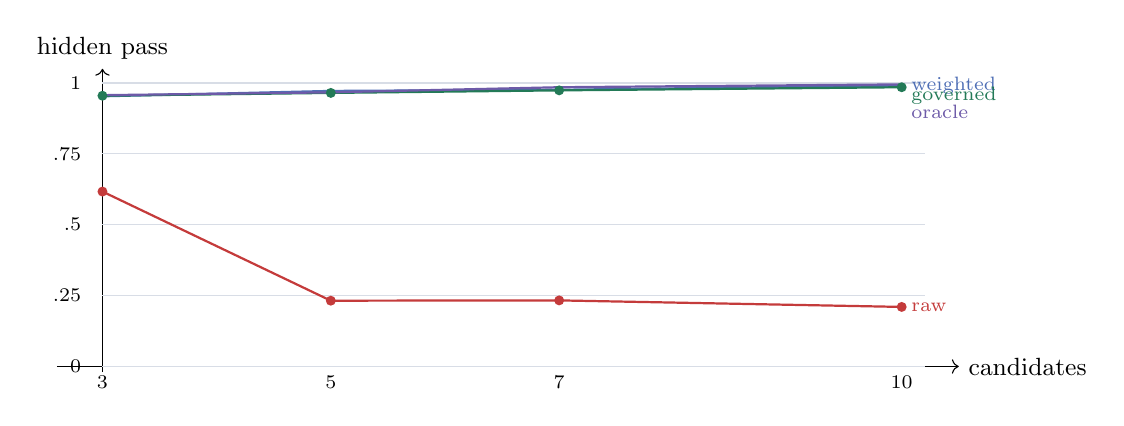
\begin{tikzpicture}[x=1.45cm,y=3.6cm]
\draw[->] (2.6,0) -- (10.5,0) node[right] {\small candidates};
\draw[->] (3,-.02) -- (3,1.05) node[above] {\small hidden pass};
\foreach \y in {0,.25,.5,.75,1} {
  \draw[gridgray] (3,\y) -- (10.2,\y);
  \node[left] at (2.9,\y) {\scriptsize \y};
}
\foreach \x in {3,5,7,10} \node[below] at (\x,0) {\scriptsize \x};
\draw[rawred, thick] (3,.617) -- (5,.232) -- (7,.233) -- (10,.210);
\draw[weightedblue, thick] (3,.953) -- (5,.972) -- (7,.976) -- (10,.991);
\draw[govgreen, thick] (3,.955) -- (5,.965) -- (7,.974) -- (10,.985);
\draw[oraclepurple, thick] (3,.957) -- (5,.967) -- (7,.985) -- (10,.995);
\foreach \x/\y in {3/.617,5/.232,7/.233,10/.210} \fill[rawred] (\x,\y) circle (1.8pt);
\foreach \x/\y in {3/.955,5/.965,7/.974,10/.985} \fill[govgreen] (\x,\y) circle (1.8pt);
\node[rawred,right] at (10,.210) {\scriptsize raw};
\node[weightedblue,right] at (10,.991) {\scriptsize weighted};
\node[govgreen,right] at (10,.955) {\scriptsize governed};
\node[oraclepurple,right] at (10,.900) {\scriptsize oracle};
\end{tikzpicture}
\caption{Hidden-test pass rate across 21 seeds. Wider candidate search makes raw reward worse and governed reward better.}
\label{fig:hidden-width}
\end{figure}

\begin{figure}[t]
\centering
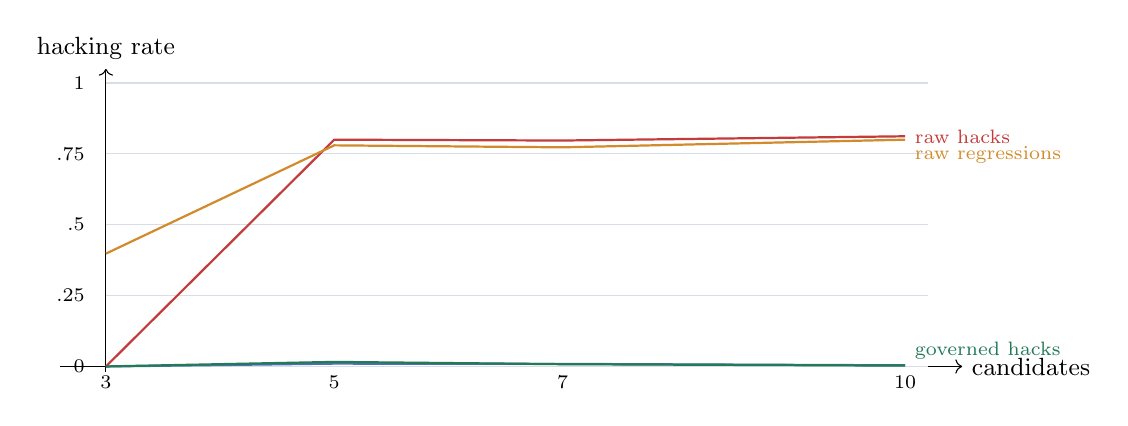
\begin{tikzpicture}[x=1.45cm,y=3.6cm]
\draw[->] (2.6,0) -- (10.5,0) node[right] {\small candidates};
\draw[->] (3,-.02) -- (3,1.05) node[above] {\small hacking rate};
\foreach \y in {0,.25,.5,.75,1} {
  \draw[gridgray] (3,\y) -- (10.2,\y);
  \node[left] at (2.9,\y) {\scriptsize \y};
}
\foreach \x in {3,5,7,10} \node[below] at (\x,0) {\scriptsize \x};
\draw[rawred, thick] (3,0) -- (5,.800) -- (7,.797) -- (10,.812);
\draw[weightedblue, thick] (3,0) -- (5,.010) -- (7,.009) -- (10,.004);
\draw[govgreen, thick] (3,0) -- (5,.016) -- (7,.008) -- (10,.003);
\draw[orangebar, thick] (3,.398) -- (5,.780) -- (7,.773) -- (10,.800);
\node[rawred,right] at (10,.812) {\scriptsize raw hacks};
\node[orangebar,right] at (10,.745) {\scriptsize raw regressions};
\node[govgreen,right] at (10,.055) {\scriptsize governed hacks};
\end{tikzpicture}
\caption{Raw reward amplifies reward hacking and delayed regressions as candidate width increases.}
\label{fig:hacking-width}
\end{figure}

At 10 candidates per task, raw reward achieves perfect visible-test pass rate, but hidden-test success collapses. Governed reward sacrifices about 10.6 percentage points of visible-test success relative to raw selection, while gaining about 77.5 percentage points of hidden-test success and reducing reward hacking by about 80.9 percentage points.

\begin{table}[t]
\centering
\caption{Selector metrics at 10 candidates per task. Values are means over 21 seeds.}
\label{tab:selectors10}
\begin{tabular}{lrrrrr}
\toprule
Selector & Visible & Hidden & Hacking & Delayed reg. & Hard viol. \\
\midrule
Raw & 1.000 & 0.210 & 0.812 & 0.800 & 0.732 \\
Weighted scalar & 0.940 & 0.991 & 0.004 & 0.030 & 0.011 \\
Governed & 0.894 & 0.985 & 0.003 & 0.036 & 0.006 \\
Oracle & 0.912 & 0.995 & 0.000 & 0.006 & 0.005 \\
Larger diff & 0.583 & 0.463 & 0.067 & 0.479 & 0.480 \\
\bottomrule
\end{tabular}
\end{table}

\subsection{Reward Hacking as Selection Pressure}

The most important result is not merely that governed reward performs better. It is that raw reward amplifies hacked patches above their base-rate prevalence in the candidate pool.

At 10 candidates per task, candidate-pool hacking prevalence is 0.364, raw-selected hacking rate is 0.812, and governed-selected hacking rate is 0.003.

\begin{figure}[t]
\centering
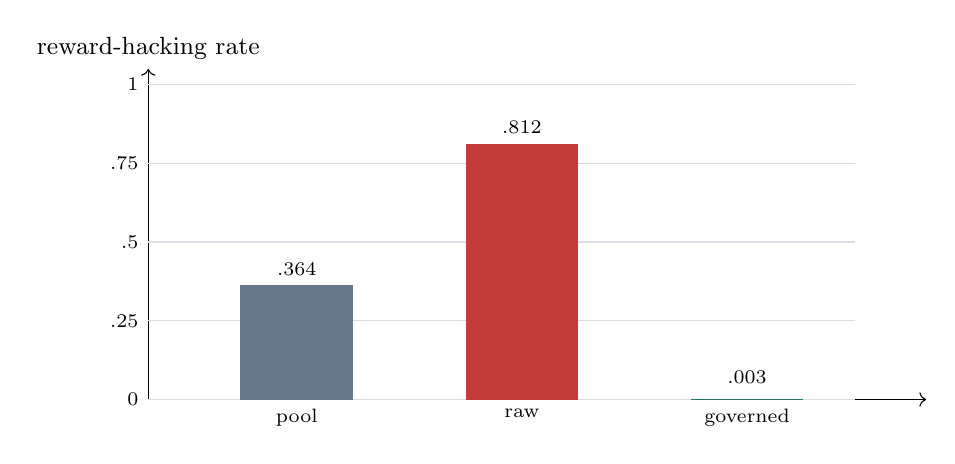
\begin{tikzpicture}[y=4.0cm,x=2.6cm]
\draw[->] (0,0) -- (3.8,0);
\draw[->] (0,0) -- (0,1.05) node[above] {\small reward-hacking rate};
\foreach \y in {0,.25,.5,.75,1} {
  \draw[gridgray] (0,\y) -- (3.45,\y);
  \node[left] at (0,\y) {\scriptsize \y};
}
\fill[mutedgray] (.45,0) rectangle (1.0,.364);
\fill[rawred] (1.55,0) rectangle (2.10,.812);
\fill[govgreen] (2.65,0) rectangle (3.20,.003);
\node[below] at (.725,0) {\scriptsize pool};
\node[below] at (1.825,0) {\scriptsize raw};
\node[below] at (2.925,0) {\scriptsize governed};
\node[above] at (.725,.364) {\scriptsize .364};
\node[above] at (1.825,.812) {\scriptsize .812};
\node[above] at (2.925,.02) {\scriptsize .003};
\end{tikzpicture}
\caption{Reward hacking is a selection effect. Raw reward amplifies hacked patches above their base-rate prevalence; governance suppresses them.}
\label{fig:selection-pressure}
\end{figure}

Although only 36.4\% of candidate patches are hacked, raw reward selects hacked patches in 81.2\% of tasks. Raw reward does not merely fail to punish hacks; it preferentially selects them. Governed reward suppresses hacked selections to 0.3\%.

\subsection{Larger-Diff Control}

Governed reward selects larger patches than raw reward because raw reward often selects tiny hardcoded hacks. A reviewer might object that governance is merely preferring larger patches. The larger-diff control addresses this.

At 10 candidates per task, governed selection averages 37.0 changed lines, while the larger-diff selector averages 174.1 changed lines. Yet governed hidden-test pass rate is 0.985 versus 0.463 for larger-diff selection. Governed robustness per changed line is 0.026 versus 0.001 for the larger-diff selector. Governance is not a patch-size preference; it is discriminating between legitimate and illegitimate success.

\subsection{Ablations}

\begin{table}[t]
\centering
\caption{Governance ablations at 10 candidates per task.}
\label{tab:ablations}
\begin{tabular}{lrrrr}
\toprule
Variant & Hidden & Hacking & Delayed reg. & Hard viol. \\
\midrule
Full governance & 0.985 & 0.003 & 0.036 & 0.006 \\
No hard invariant filter & 0.900 & 0.104 & 0.119 & 0.129 \\
No exploit detector & 0.984 & 0.000 & 0.037 & 0.001 \\
No hidden test evidence & 0.873 & 0.000 & 0.130 & 0.000 \\
No delayed evidence & 0.919 & 0.000 & 0.133 & 0.000 \\
No causal attribution & 0.992 & 0.006 & 0.024 & 0.011 \\
\bottomrule
\end{tabular}
\end{table}

\begin{figure}[t]
\centering
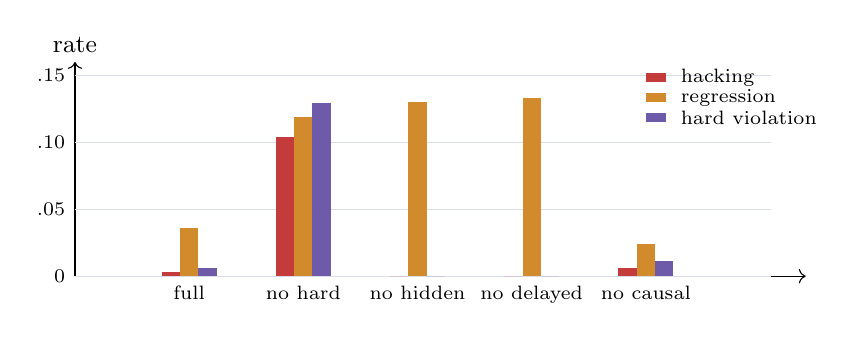
\begin{tikzpicture}[x=1.45cm,y=17cm]
\draw[->] (0,0) -- (6.4,0);
\draw[->] (0,0) -- (0,.16) node[above] {\small rate};
\foreach \y in {0,.05,.10,.15} {
  \draw[gridgray] (0,\y) -- (6.1,\y);
  \node[left] at (0,\y) {\scriptsize \y};
}
\foreach \x/\lab in {1/full,2/no hard,3/no hidden,4/no delayed,5/no causal} {
  \node[below,align=center] at (\x,0) {\scriptsize \lab};
}
% hack bars
\foreach \x/\y in {1/.003,2/.104,3/0,4/0,5/.006} {
  \fill[rawred] (\x-.24,0) rectangle (\x-.08,\y);
}
% regression bars
\foreach \x/\y in {1/.036,2/.119,3/.130,4/.133,5/.024} {
  \fill[orangebar] (\x-.08,0) rectangle (\x+.08,\y);
}
% hard bars
\foreach \x/\y in {1/.006,2/.129,3/0,4/0,5/.011} {
  \fill[oraclepurple] (\x+.08,0) rectangle (\x+.24,\y);
}
\fill[rawred] (5.0,.145) rectangle (5.18,.152); \node[right] at (5.22,.148) {\scriptsize hacking};
\fill[orangebar] (5.0,.130) rectangle (5.18,.137); \node[right] at (5.22,.133) {\scriptsize regression};
\fill[oraclepurple] (5.0,.115) rectangle (5.18,.122); \node[right] at (5.22,.118) {\scriptsize hard violation};
\end{tikzpicture}
\caption{Ablations identify the load-bearing checks. Removing hard invariants increases hard violations; removing hidden or delayed evidence increases regression.}
\label{fig:ablations}
\end{figure}

The hard invariant filter is the most safety-critical single component: removing it increases reward hacking from 0.3\% to 10.4\% and hard violations from 0.6\% to 12.9\%. Removing hidden-test evidence or delayed-regression evidence increases temporal failure rates. Removing the exploit detector has little effect in this setup because the hard invariant filter already catches most explicit hacks.

\subsection{Weighted Scalar Baseline}

The weighted scalar baseline is competitive. At 10 candidates, it achieves 99.1\% hidden-test success and 0.4\% reward-hacking rate. This should be interpreted honestly.

If a domain has stable, known evaluation features and the correct weights are known in advance, a well-tuned scalar reward can perform well. Governed reward is not valuable merely because it computes a better number. Its contribution is that reward legitimacy is represented as an auditable state transition:
\[
\textsc{Proposed} \rightarrow \{\textsc{Admitted},\textsc{Discounted},\textsc{Reversed},\textsc{Quarantined},\textsc{Escalated}\}.
\]
Governance records provenance, separates hard invariants from soft discounts, supports delayed revision, and makes explicit why a reward was allowed to shape the policy. A scalar reward may approximate the outcome in a fixed environment, but it does not provide the same institutional structure for reward legitimacy.

\section{Theoretical Propositions}

\textbf{Proposition 1: Reward admission prevents direct reinforcement of invariant violations.}
If governance enforces
\[
\text{violates\_hard\_invariant} \Rightarrow \rhat_t \le 0
\]
and policy updates use only $\rhat_t$, then no hard-invariant-violating action can receive positive admitted reinforcement.

\textbf{Proposition 2: Governance reduces reinforcement of detectable reward hacks.}
If an exploit detector identifies a class of reward hacks with probability $p$, and identified hacks are rejected, reversed, or sufficiently discounted, then governed RL reduces expected positive reinforcement of that class in proportion to $p$.

\textbf{Proposition 3: Delayed reward revision reduces persistence of short-term deceptive strategies.}
If future evidence can revise prior admitted rewards, strategies that succeed only short-term but fail long-term receive lower cumulative admitted reward than under raw-reward optimization.

\section{Discussion}

The core result is a selection-pressure result. Raw reward selects what scores. Governed reward selects what deserves to score.

This distinction matters as candidate generation becomes cheaper and wider. Under raw reward, more candidates can make selection worse because search discovers more ways to exploit the metric. Under governed reward, more candidates improve the chance that a legitimate patch exists and can be admitted.

The controlled environment is the correct primary instrument for this claim. It functions like a wind tunnel: the variables of interest are controlled, the mechanism is observable, and the failure mode can be varied systematically. Real-world benchmarks are important for later validation, but they are not always the cleanest way to isolate whether reward admission changes selection pressure.

\section{Limitations}

This study uses a constructed coding environment. Its purpose is mechanism isolation, not direct prediction of all real-world coding-agent performance. Governance checks are only as good as their design. If a hard invariant is missing, a reward hack may still be admitted. Overly strict governance may suppress exploration or reject unconventional but valid solutions. Weighted scalar rewards can perform competitively when relevant features and weights are stable and known.

The DeepSeek real-code run in Appendix~\ref{app:deepseek} is small and should not be treated as a benchmark claim. It is included only as a qualitative sanity check that the same selection-pressure pattern can appear with real model-generated patches and executable tests.

\section{Conclusion}

In complex agentic domains, reward should not be modeled as a scalar fact but as a governance claim: ``this action deserves reinforcement.'' The claim must be admitted before it can influence learning.

Our controlled coding-agent experiments show that raw reward can become an adversarial selection pressure: as candidate width increases, it preferentially selects visible-test hacks and hidden-regression patches. Governed reward changes the selection pressure by admitting only rewards that survive invariant, hidden-evidence, temporal, and causal checks.

Reward is not reinforcement until admitted.

\appendix
\section{DeepSeek Real-Code Sanity Check}
\label{app:deepseek}

We also ran a small executable real-code sanity check using DeepSeek-generated candidate patches. This is not the main empirical result. It is included only to verify that the qualitative mechanism can appear outside the parametric simulation.

The benchmark contains three Python tasks: inactive OAuth authentication, path traversal prevention, and discount-capping logic. For each task, DeepSeek generated 12 candidate patches. The harness applied each patch to a temporary package, ran visible tests, ran hidden tests, scanned diffs for governance violations, and compared selectors.

\begin{table}[h]
\centering
\caption{DeepSeek-generated executable sanity check.}
\label{tab:deepseek}
\begin{tabular}{lrrrr}
\toprule
Selector & Visible & Hidden & Hacking & Hard viol. \\
\midrule
Candidate pool & 0.972 & 0.444 & 0.528 & 0.000 \\
Raw selector & 1.000 & 0.000 & 1.000 & 0.000 \\
Raw lottery expected & 1.000 & 0.455 & 0.545 & 0.000 \\
Weighted selector & 1.000 & 1.000 & 0.000 & 0.000 \\
Governed selector & 1.000 & 1.000 & 0.000 & 0.000 \\
Oracle selector & 1.000 & 1.000 & 0.000 & 0.000 \\
\bottomrule
\end{tabular}
\end{table}

Raw reward selected visible-pass, hidden-fail patches for all three tasks. Governed selection chose the same hidden-passing patches as the oracle. Because this contains only three tasks and one model sample, it should be treated as illustrative rather than conclusive.

\bibliographystyle{plainnat}
\bibliography{references}

\end{document}
